% \bibliography{../src/bibliography.bib}

Throughout these note we write $x$ for a sentence, $y$ for a (latent) constituency tree, and $\mathcal{Y}(x)$ for the \textit{yield} of $x$, that is, all trees that can be assigned to $x$. Furthermore, let $\mathbb{L}$ be a set of pairs $(x, y)$ of sentences with gold trees, and let $\mathbb{U}$ be a set of unlabeled sentences $x$.

We define the following semi-supervised objective
\begin{align*}
    \mathcal{J} \triangleq \mathcal{J}_{\mathcal{S}} + \alpha \mathcal{J}_{\mathcal{U}},
\end{align*}
were $\mathcal{J}_{\mathcal{S}}$ is the supervised objective optimized over $\mathbb{L}$ and $\mathcal{J}_{\mathcal{U}}$ the unsupervised objective optimized over $\mathbb{U}$. We introduce $\alpha \in \mathbb{R}$ as an arbitrary scalar controlling the contribution of the unsupervised objective.

\section{Supervised objective}
Let $p_{\theta}(x,y)$ be parametrized by a Generative RNNG \citep{Dyer+2016:RNNG}. Then our supervised objective is
\begin{align*}
    \mathcal{J}_{\mathcal{S}}
        &\triangleq \sum_{(x,y) \in \mathbb{L}} \log p_{\theta} (x, y) \\
\end{align*}
This objective is optimized as usual using stochastic gradient estimates:
\begin{align*}
    \nabla_{\theta} \mathcal{J}_{\mathcal{S}}
        &\approx \frac{|\mathbb{L}|}{n} \sum_{i=1}^n \nabla_{\theta} \log p_{\theta} (x^{(i)}, y^{(i)}), \\
\end{align*}
where $\{(x^{(i)}, y^{(i)})\}_{i=1}^n$ is a mini-batch sampled uniformly from $\mathbb{L}$. To compute $\nabla_{\theta} \log p_{\theta}(x^{(i)}, y^{(i)})$ we rely on automatic differentiation \citep{Baydin+2017:AD}.

\section{Unsupervised objective}
Consider the following objective to be maximized:
\begin{subequations}
\begin{align*}
    \mathcal{J}_{\mathcal{U}}
        &\triangleq \sum_{x \in \mathbb{U}} \log p (x) \\
        &= \sum_{x \in \mathbb{U}} \log \sum_{y \in \mathcal{Y}(x)} p_{\theta}(x, y)
\end{align*}
\end{subequations}
This is a language modelling objective, in which we treat $y$ as latent, and $p_{\theta}(x,y)$ is a generative RNNG. A consequence the independence assumptions of the RNNG (or better: lack thereof) is that the sum over trees $y$ is no longer tractable.  To optimize this objective we must fall back on approximate methods.

\paragraph{Variational approximation} We optimize the objective using variational inference \citep{Blei+2016:VI}. We introduce a posterior $q_{\lambda}(y|x)$ parametrised by $\lambda$ and use Jensen's inequality to derive a variational lower bound:
\begin{subequations}
\begin{align*}
    \log p (x)
        &= \log \sum_{y \in \mathcal{Y}(x)} q_{\lambda}(y|x) \frac{p_{\theta}(x, y)}{q_{\lambda}(y|x)} \\
        &= \log \mathbb{E}_{q_{\lambda}} \bigg[\frac{p_{\theta}(x, y)}{ q_{\lambda}(y|x)} \bigg] \\
        &\geq \mathbb{E}_{q_{\lambda}} \bigg[\log \frac{p_{\theta}(x, y)}{q_{\lambda}(y|x)} \bigg] \\
        &= \mathbb{E}_{q_{\lambda}} \big[\log p_{\theta}(x, y)  - \log q_{\lambda}(y|x) \big] \triangleq \mathcal{L}(\theta, \lambda)
\end{align*}
\end{subequations}
The only requirement for $q_{\lambda}$ is that
\begin{align*}
    p(x,y) > 0 \Rightarrow q(y|x) > 0 \qquad \text{for all $x$ and $y \in \mathcal{Y}(x)$}.
\end{align*}
Any discriminatively trained parser fulfills this requirement.

The lower bound $\mathcal{L}(\theta, \lambda)$ will be optimized by gradient optimization, which means we will need to take the gradients $\nabla_{\theta} \mathcal{L}(\theta, \lambda)$ and $\nabla_{\lambda} \mathcal{L}(\theta, \lambda)$.

\paragraph{Gradients of joint parameters} The first gradient is easy and permits a straightforward Monte-Carlo estimate:
\begin{subequations}
\begin{align*}
    \nabla_{\theta} \mathcal{L}(\theta, \lambda)
        &= \nabla_{\theta} \mathbb{E}_{q_{\lambda}} \big[\log p_{\theta}(x, y)  - \log q_{\lambda}(y|x) \big] \\
        &= \mathbb{E}_{q_{\lambda}} \big[ \nabla_{\theta} \log p_{\theta}(x, y)  -  \nabla_{\theta} \log q_{\lambda}(y|x) \big] \\
        &= \mathbb{E}_{q_{\lambda}} \big[ \nabla_{\theta} \log p_{\theta}(x, y) \big] \\
        &\approx \frac{1}{n}\sum_{i=1}^n  \nabla_{\theta} \log p_{\theta}(x, y^{(i)})
\end{align*}
\end{subequations}
where $y_i \sim q_{\lambda}(y|x)$ for $i=1,\dots,n$. We can move the gradient inside the expectation (second equality) because $q$ does not depend on $\theta$.

\paragraph{Gradients of posterior parameters}
The second gradient is harder and requires us to rewrite the objective:
\begin{subequations}
\begin{align*}
\nabla_{\lambda} \mathcal{L}(\theta, \lambda)
        &= \nabla_{\lambda} \mathbb{E}_{q_{\lambda}} \big[\log p_{\theta}(x, y)  - \log q_{\lambda}(y|x) \big] \\
        &= \nabla_{\lambda} \sum_{y} \big\{ q_{\lambda}(y|x) \log p_{\theta}(x, y) - q_{\lambda}(y|x)\log q_{\lambda}(y|x) \big\} \\
        &= \sum_{y} \big\{ \nabla_{\lambda} q_{\lambda}(y|x) \log p_{\theta}(x, y) \\
        &\qquad\qquad - \nabla_{\lambda} q_{\lambda}(y|x)\log q_{\lambda}(y|x) \\
        &\qquad\qquad -  q_{\lambda}(y|x)\nabla_{\lambda}\log q_{\lambda}(y|x) \big\} \\
        &= \sum_{y} \big\{ \nabla_{\lambda} q_{\lambda}(y|x) \log p_{\theta}(x, y) - \nabla_{\lambda} q_{\lambda}(y|x)\log q_{\lambda}(y|x) \big\} \\
        &= \sum_{y} \big\{(\log p_{\theta}(x, y) - \log q_{\lambda}(y|x))\nabla_{\lambda} q_{\lambda}(y|x) \big\} \\
        &= \sum_{y} \big\{(\log p_{\theta}(x, y) - \log q_{\lambda}(y|x)) q_{\lambda}(y|x)\nabla_{\lambda} \log q_{\lambda}(y|x) \big\}   \\
        &= \mathbb{E}_{q_{\lambda}} \big[ (\log p_{\theta}(x, y) - \log q_{\lambda}(y|x))  \nabla_{\lambda} \log q_{\lambda}(y|x) \big\} \\
        &= \mathbb{E}_{q_{\lambda}} \big[ l(x, y) \nabla_{\lambda} \log q_{\lambda}(y|x) \big]
\end{align*}
\end{subequations}
Where we've defined a learning signal $l(x, y) \triangleq \log p_{\theta}(x, y) - \log q_{\lambda}(y|x)$.

In this derivation we used the identity
\begin{align*}
    \nabla_{\lambda}\log q_{\lambda}(y|x) &= \frac{\nabla_{\lambda} q_{\lambda}(y|x)}{q_{\lambda}(y|x)}
\end{align*}
or equivalently
\begin{align*}
    \nabla_{\lambda} q_{\lambda}(y|x) &= q_{\lambda}(y|x)\nabla_{\lambda}\log q_{\lambda}(y|x)
\end{align*}
and the fact that
\begin{subequations}
\begin{align*}
    \sum_{y} q_{\lambda}(y|x)\nabla_{\lambda}\log q_{\lambda}(y|x)
        &= \sum_{y}  q_{\lambda}(y|x) \frac{\nabla_{\lambda} q_{\lambda}(y|x)}{q_{\lambda}(y|x)}  \\
        &= \sum_{y} \nabla_{\lambda} q_{\lambda}(y|x) \\
        &= \nabla_{\lambda} \sum_{y} q_{\lambda}(y|x)\\
        &= \nabla_{\lambda} 1 \\
        &= 0. \\
\end{align*}
\end{subequations}

This rewritten objective permits a straightforward MC estimate:
\begin{align}
\label{eq:score-function-estimator}
    \mathbb{E}_{q_{\lambda}} \big[ l(x,y) \nabla_{\lambda} \log q_{\lambda}(y|x) \big]
        &\approx \frac{1}{n}\sum_{i=1}^n  l(x,y^{(i)})\nabla_{\lambda} \log q_{\lambda}(x|y^{(i)})
\end{align}
where $y_i \sim q_{\lambda}(y|x)$ for $i=1,\dots,n$.

This estimator has been derived (in slightly different forms) in among others \citep{Williams1992:REINFORCE}, \citep{Paisley+2012:VISS}, \citep{Mnih+2014:NVIL}, \citep{Ranganath+2014:BBVI}, and \citep{Miao+2016} and is known as the \textsc{reinforce} estimator \citep{Williams1992:REINFORCE}, or score function estimator (after the score function $\nabla_{\theta} \log p_{\theta}(x)$) \citep{Fu2006}.

\section{Optimization}
We use automatic differentiation \citep{Baydin+2017:AD} to obtain all our gradient estimates.

To get the gradients in formula \ref{eq:score-function-estimator} we rewrite it in the form of a surrogate objective \citep{Schulman+2015:surrogate}
\begin{align*}
    L(\lambda) &= \frac{1}{n}\sum_{i=1}^n \log q_{\lambda}(x|y^{(i)}) \textsc{blockgrad}(l(x,y^{(i)}))
\end{align*}
where \textsc{blockgrad} is function that `detaches' a parametrized function from the computation graph effectively turning it into a scalar. That is, loosely speaking
\begin{align*}
    \textsc{blockgrad}(f_{\theta}(x)) &= f(x)
\end{align*}
such that
\begin{align*}
    \nabla_{\theta}\textsc{blockgrad}(f_{\theta}(x)) &= \nabla_{\theta} f(x) \\
        &= 0
\end{align*}
Then differentiation of $L$ gives us the unbiased estimator
\begin{align*}
    \nabla_{\lambda} L(\lambda) &= \frac{1}{n}\sum_{i=1}^n l(x,y^{(i)}) \nabla_{\lambda} \log q_{\lambda}(x|y^{(i)})
\end{align*}

\section{Variance reduction}
We have derived an estimator for the gradient of the posterior parameters in the unsupervised objective. This estimator is unbiased, but is known to have high variance, often too much to be useful \citep{Paisley+2012:VISS}. Two effective methods to counter this are control variates and baselines \citep{Ross:2006:SIM}.

\paragraph{Variance of estimator} First, let's analyze the variance of our estimator. Note that our expectation is of the general form
\begin{align*}
    \mu \triangleq \mathbb{E}\big[f(X)\big]
\end{align*}
and that we estimate this quantity by generating $n$ independent samples $X_1,\dots,X_n \sim P(X)$ and computing
\begin{align*}
    \hat{\mu} \triangleq \frac{1}{n} \sum_{i=1}^n f(X_i).
\end{align*}
This is an unbiased estimator for $\mu$ with error
\begin{align*}
    \text{MSE} = \mathbb{E}\big[(\mu - \hat{\mu})^2\big] &= \text{Var}[ \hat{\mu} ] = \frac{\text{Var}[ \hat{\mu} ]}{n},
\end{align*}
which means that the error is of the order
\begin{align*}
    \mu - \hat{\mu} \sim \sqrt{\frac{\text{Var}[ \hat{\mu} ]}{n}}
\end{align*}
and reducing it linearly requires a quadratic number of samples.

In our particular case, the function $f$ is
\begin{align*}
    f_{X=x}(Y) &\triangleq l(X,Y) \nabla_{\lambda} \log q_{\lambda}(Y|X=x)
\end{align*}
where we have made explicit that $y$ is the random variable, and $x$ is given.

\paragraph{Control variates} Consider a function $\phi(X)$ with known expectation
\begin{align*}
    \mu_{\phi} \triangleq \mathbb{E} [ \phi(X) ]
\end{align*}
Then we can define a new function $\hat{f}$ such that
\begin{align*}
    \hat{f}(X) \triangleq f(X) - \phi(X) + \mu_{\phi}.
\end{align*}
This function is also an estimator for $\mu$, since
\begin{align*}
    \mathbb{E}[ \hat{f}(X) ] &= \mathbb{E}[ f(X) ] - \mu_{\phi} + \mu_{\phi} \\
        &= \mathbb{E}[ f(X) ],
\end{align*}
and a computation shows that the variance of the new function is
\begin{align*}
    \text{Var}[ \hat{f}(X) ] &= \mathbb{E}[ (f(X) - \phi(X) + \mu_{\phi}) - \mu)^2 ] \\
    &= \mathbb{E}[ (f(X) - \phi(X) + \mu_{\phi})^2 ] - 2\mathbb{E}[ (f(X) - \phi(X) + \mu_{\phi})\mu ] + \mathbb{E}[ \mu^2 ] \\
    &= \mathbb{E}[ (f(X) - \phi(X) + \mu_{\phi})^2 ] - 2\mathbb{E}[ (f(X) - \phi(X) + \mu_{\phi})]\mu + \mu^2 \\
    &= \mathbb{E}[ (f(X) - \phi(X) + \mu_{\phi})^2 ] - 2\mu^2  + \mu^2 \\
    &= \mathbb{E}[ f(X)^2 + \phi(X)^2 + \mu_{\phi}^2 - 2f(X)\phi(X) + 2f(X)\mu_{\phi} - 2\phi(X)\mu_{\phi} ] - \mu^2\\
    % &= \mathbb{E}[ f(X)^2 + \phi(X)^2 + \mathbb{E}[ \phi(x) ] ^2 - 2f(X)\phi(X) + 2f(X)\mathbb{E}[ \phi(x) ] - 2\phi(X)\mathbb{E}[ \phi(x) ] ] - \mathbb{E}[ f(X) ]^2\\
    &= \mathbb{E}[ f(X)^2 ] - \mathbb{E}[ f(X) ]^2 \\
    &\quad - 2(\mathbb{E}[ f(X)\phi(X) ] - \mathbb{E}[ f(X) ]\mathbb{E}[ \phi(X) ]) \\
    &\quad+ \mathbb{E}[ \phi(X)^2 ] - \mathbb{E}[ \phi(X) ]^2 \\
    &= \text{Var}[ f(X) ] - 2 \text{ Cov}[ f(X), \phi(X) ] + \text{Var}[ \phi(X) ]
\end{align*}
This means we can get a reduction in variance whenever
\begin{align*}
    \text{Cov}[ f(X), \phi(X) ] > \frac{1}{2}\text{ Var}[ \phi(X) ].
\end{align*}
The function $\phi$ is called a \textit{control variate}---it allows us to control the variance of $f$.

From the equality above we can see that this will be the case whenever $f(X)$ and $\phi(X)$ are strongly correlated. Our choice of control variate will be made with the that in mind. Furthermore, $\mathbb{E}[ \phi(X) ]$ must be known. What is an optimal control variate? Typically a control variate of the form $a\phi$ is chosen with fixed, and $a$ is optimized to maximize the correlation. This brings us to the generic formulation of a control variate:
\begin{align*}
    \hat{f}(X) \triangleq f(X) - a(\phi(X) - \mathbb{E}[ \phi(X) ])
\end{align*}
with variance
\begin{align*}
    \text{Var}[ \hat{f}(X) ] &= \text{Var}[ f(X) ] - 2a \text{ Cov}[ f(X), \phi(X) ] + a^2\text{ Var}[ \phi(X) ] \\
\end{align*}
We take a derivative of this with respect to $a$
\begin{align*}
    \frac{\partial}{\partial a}\text{Var}[ \hat{f}(X) ] &= - 2 \text{ Cov}[ f(X), \phi(X) ] + 2a\text{ Var}[ \phi(X) ]
\end{align*}
Setting this to zero and solving for $a$ we obtain the optimal choice for $a$
\begin{align}
\label{eq:cv-scale}
    a &= \frac{\text{ Cov}[ f(X), \phi(X) ]}{\text{ Var}[ \phi(X) ]}.
\end{align}

Plugging in this solution into the expression for $\text{Var}[ \hat{f}(X) ]$ and dividing by $\text{Var}[ f(X) ]$ we get
\begin{align}
\label{eq:var-red}
    \frac{\text{Var}[ \hat{f}(X) ]}{\text{Var}[ f(X) ]} &= 1 - \frac{\text{Cov}[ f(X), \phi(X) ]}{\text{ Var}[ f(X) ] \text{ Var}[ \phi(X) ]} \\
        &= 1 - \text{corr}^2[ f(X), \phi(X) ],
\end{align}
which shows that given this choice of $a$ the reduction in variance is directly determined by the correlation between $f(X)$ and $\phi(X)$.

Bringing this all together, we let our new estimator be
\begin{align*}
    \mathbb{E}[ f(X) ] &= \mathbb{E}[ \hat{f}(X) ] \approx \frac{1}{n} \sum_{i=1}^n [ f(X_i) - a\phi(X_i) ] - \mu_{\phi}
\end{align*}

\paragraph{Example} \citep{Ross:2006:SIM} Suppose we want to use simulation to determine
\begin{align*}
    \mathbb{E}[f(X)] &= \mathbb{E}[e^X] = \int_0^1 e^x dx = e - 1
\end{align*}
with $X \sim \mathcal{U}(0,1)$. A natural control variate to use in this case is the random variable $X$ itself: $\phi(X) \triangleq X$. We thus define the new estimator
\begin{align*}
    \hat{f}(X) &= f(X) - \phi(X) + \mathbb{E}[ \phi(X) ] \\
        &= e^X - X + \frac{1}{2}.
\end{align*}

To compute the decrease in variance with this new estimator, we first note that
\begin{align*}
    \text{Cov}(e^X, X) &= \mathbb{E}[ Xe^X ] - \mathbb{E}[ X ]\mathbb{E}[ e^X ] \\
        &= \int_0^1 xe^x dx - \frac{e-1}{2} \\
        &= 1 - \frac{e-1}{2} \approx 0.14086 \\
    \text{Var}[e^X] &= \mathbb{E}[e^{2X}] - (\mathbb{E}[e^X])^2 \\
        &= \int_0^1 e^{2x} dx - (1 - e^x)^2 \\
        &= \frac{e^2 - 1}{2}  - (1 - e^x)^2 \approx 0.2420 \\
    \text{Var}[X] &= \mathbb{E}[X^2] - (\mathbb{E}[X])^2 \\
        &= \int_0^1 x^2 dx - \frac{1}{4} \\
        &= \frac{1}{3} - \frac{1}{4} = \frac{1}{12}.
\end{align*}
When we choose $a$ as in formula \ref{eq:cv-scale} we can use formula \ref{eq:var-red} to compute that
\begin{align*}
    \frac{\text{Var}[ \hat{f}(X) ]}{\text{Var}[ f(X) ]} &= 1 - \frac{(0.14086)^2}{\frac{0.2420}{12}} \\
        &\approx 0.0161.
\end{align*}
This is a reduction of 98.4 percent! A simulation illustrates what this looks like in practice with \dots samples:
\begin{figure}
  \center
  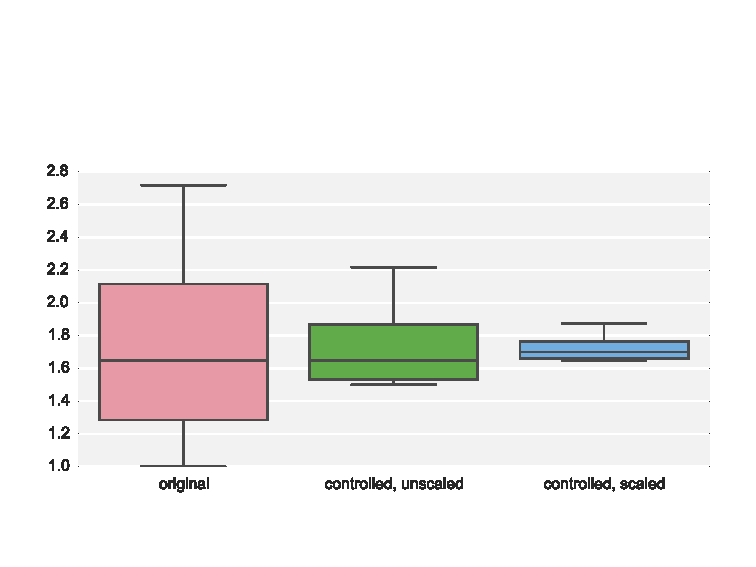
\includegraphics[width=0.7\textwidth]{control-variate.pdf}
\end{figure}
